\chapter{Практика}
\label{ch:chap2}

\subsection*{Задание 1: Для временных функций s1(t) и h(t) задайте временные параметры и выполните по шагам вычисление интеграла свертки задавая пределы интегрирования}

\begin{figure}[H]
    \centering
    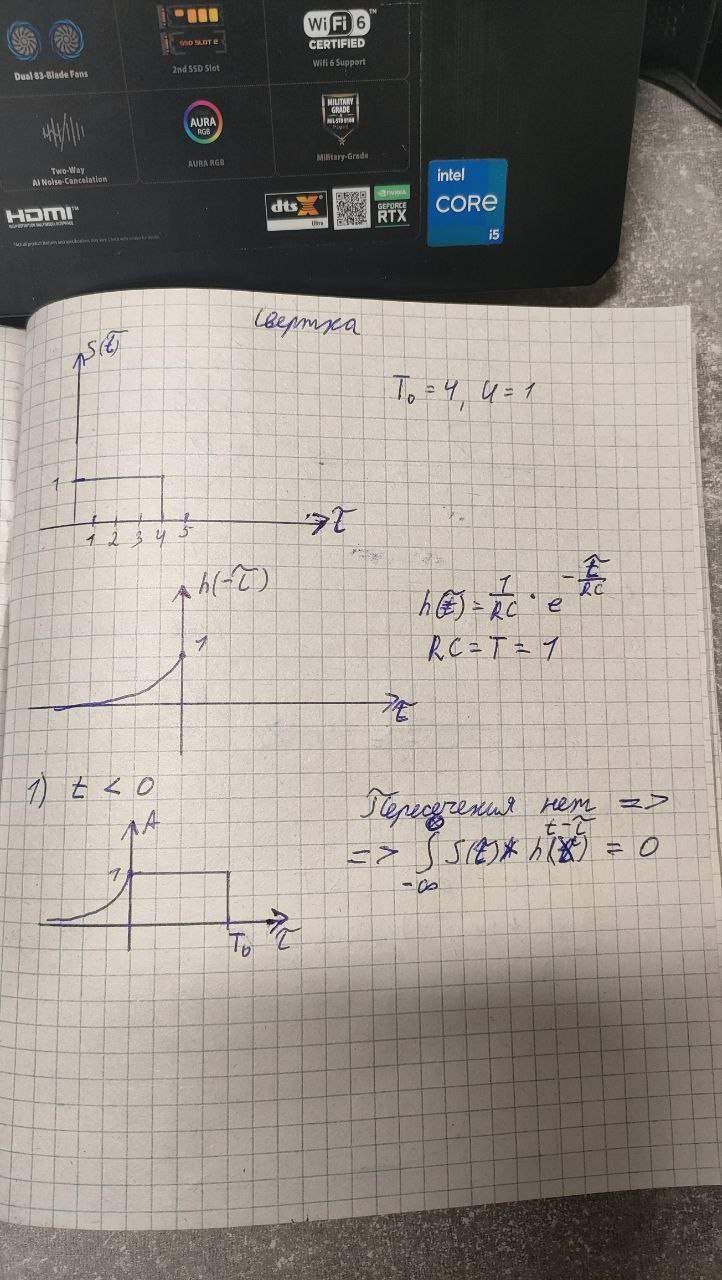
\includegraphics[width=1.0\textwidth]{hw1.png}
    \caption{Задание 1}
\end{figure}

\begin{figure}[H]
    \centering
    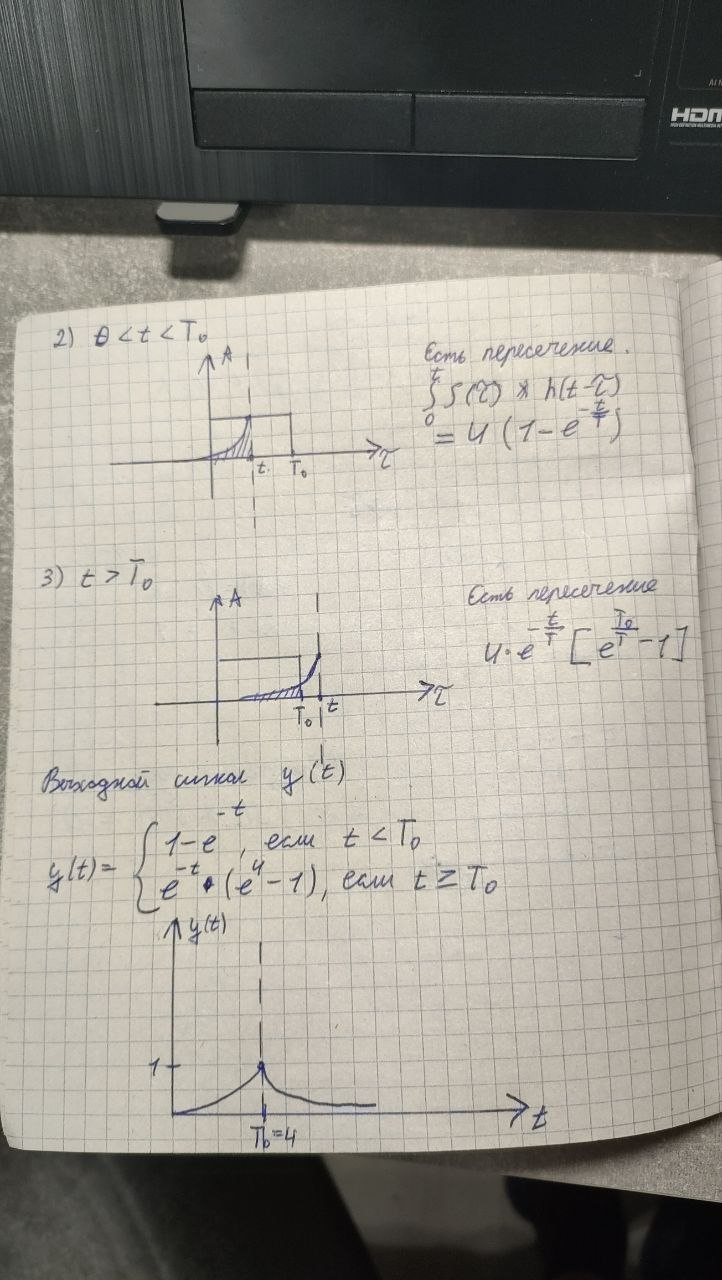
\includegraphics[width=1.0\textwidth]{hw2.png}
    \caption{Задание 2}
\end{figure}

\subsection*{Задание 2:  Вычисление инеграла свертки численным интегрированием}

Сформируем прямоугольный сигнал и импульсную характеристику RC-цепи

\begin{figure}[H]
    \centering
    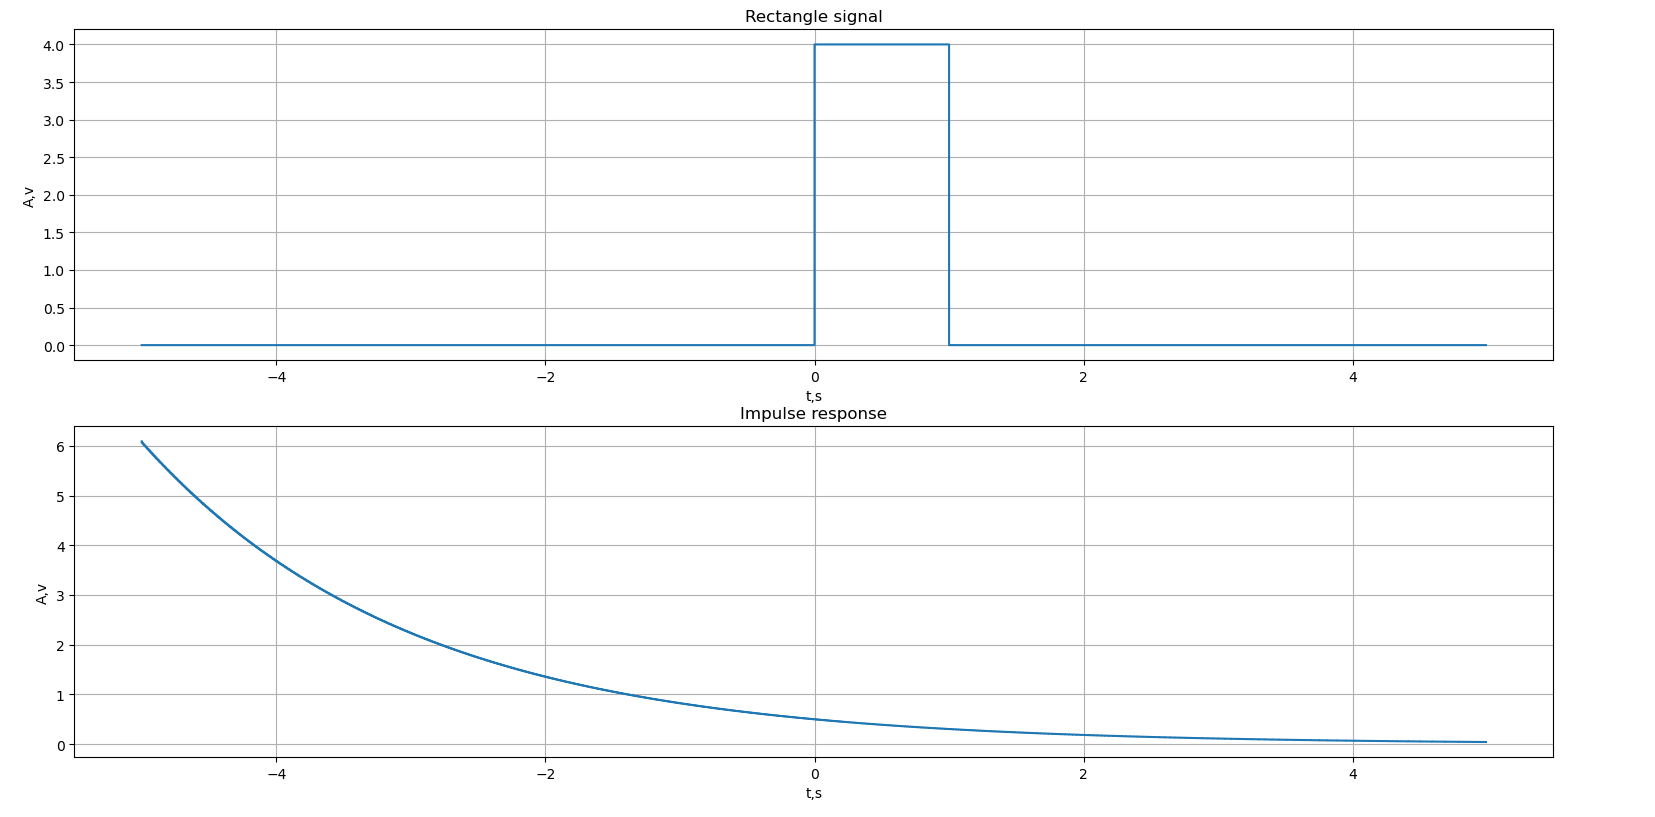
\includegraphics[width=1.0\textwidth]{rectandh.png}
    \caption{График прямоугольного сигнала и импульсная характеристика RC-цепи}
\end{figure}

Сдвинем прямоугольный сигнал на t = [-1, 0, 2]. Визуализируем сдвиг. Для каждого сдвинутого сигнала найдем $\int_{-5}^{5}h(\tau)s(t-\tau)$ путем
численного интегрирования.

\begin{figure}[H]
    \centering
    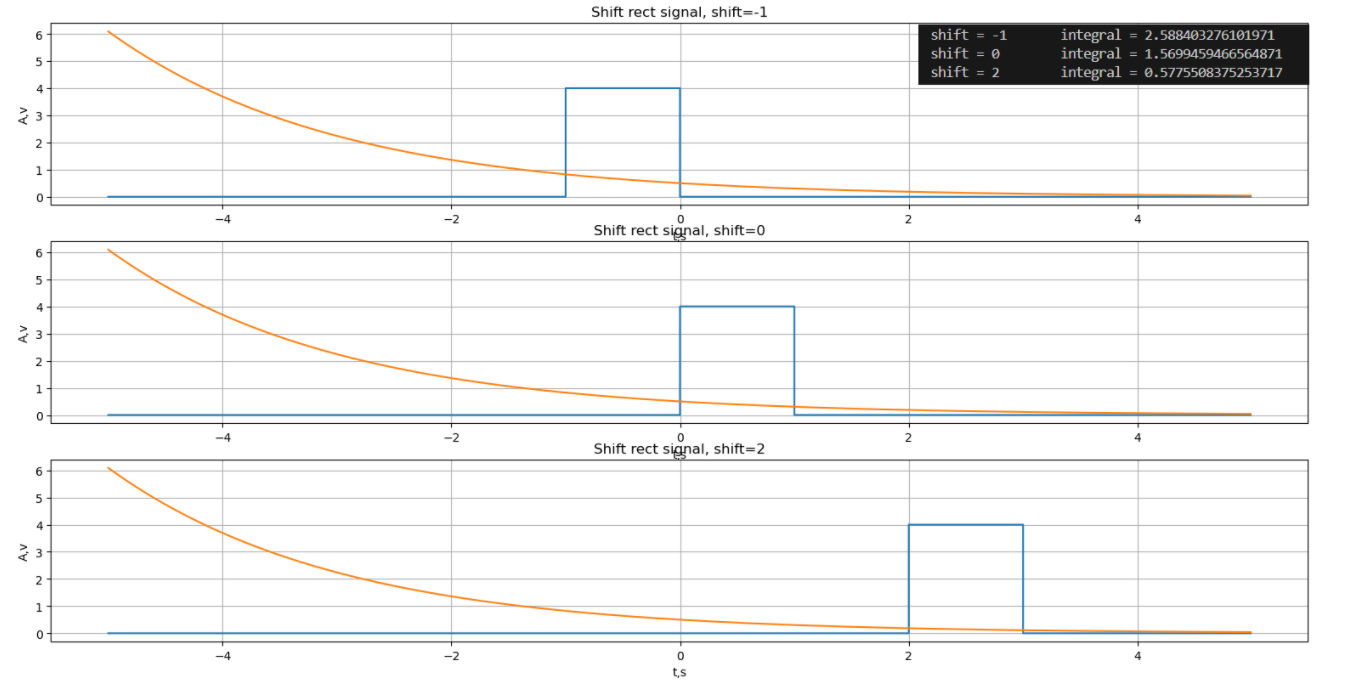
\includegraphics[width=1.0\textwidth]{shift.png}
    \caption{Сдвиг прямоугольного сигнала}
\end{figure}

При отрицательных t график сдвигается влево, при положительных - вправо. При сдвиге вправо пересечением между графиками уменьшается
и площадь тоже уменьшается.\\

Проделаем те же действия, но при $t \in (-10, 10)$

\begin{figure}[H]
    \centering
    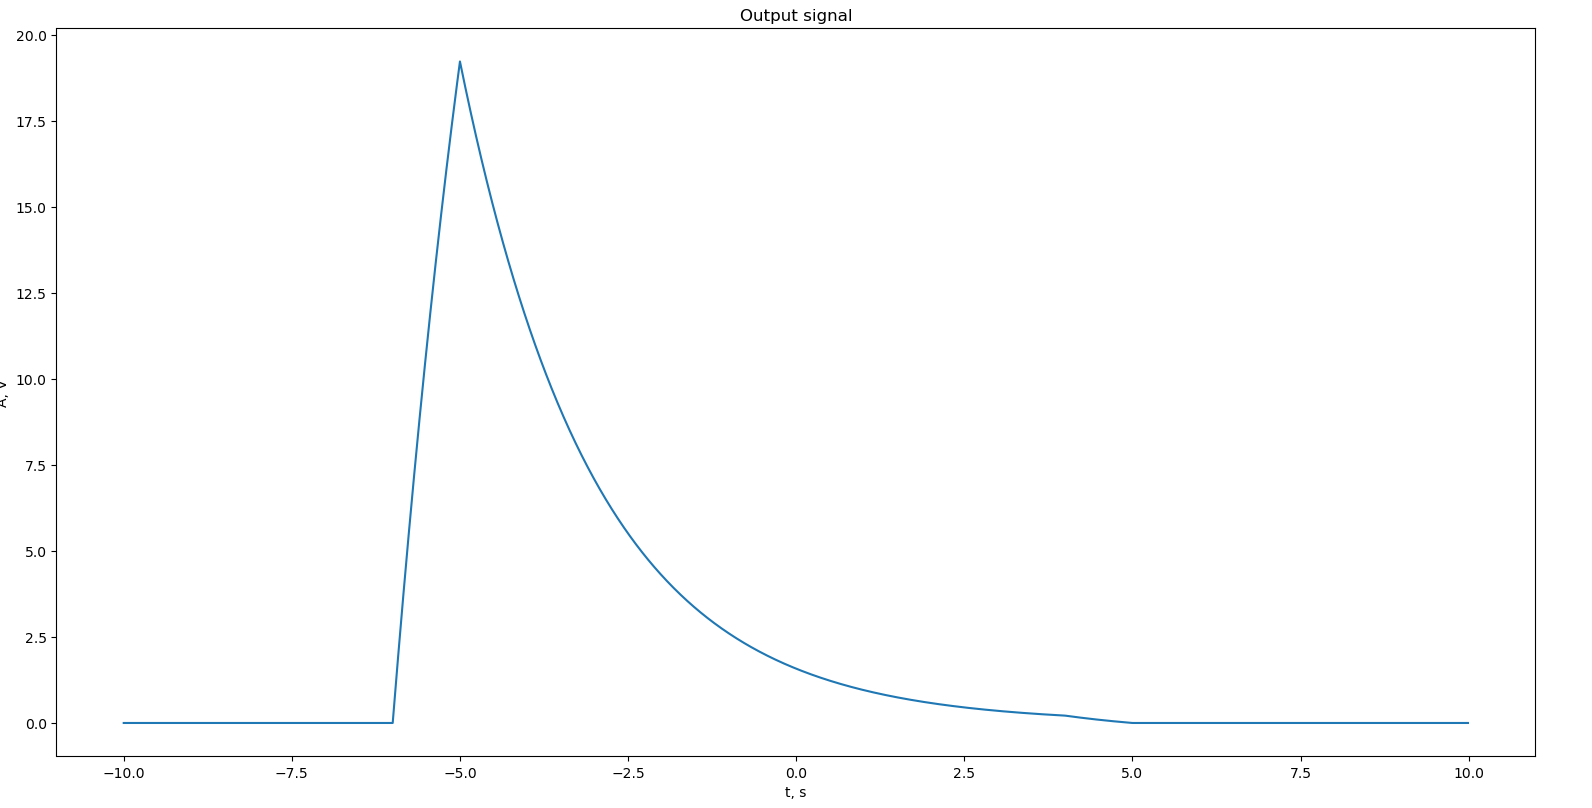
\includegraphics[width=1.0\textwidth]{yt.png}
    \caption{Реакция RC-цепи на прямоугольный импульс}
\end{figure}

При таких сдвигах прямоугольного сигнала полностью проходит через h(t) и получается реакция системы на прямоугольный сигнал.

\endinput